\section{Decision Trees}

Decision trees involve breaking down a dataset into smaller and smaller subsets. The result of this is a tree like structure containing decision nodes and leaf nodes.

\begin{figure}[H]
  \centering
  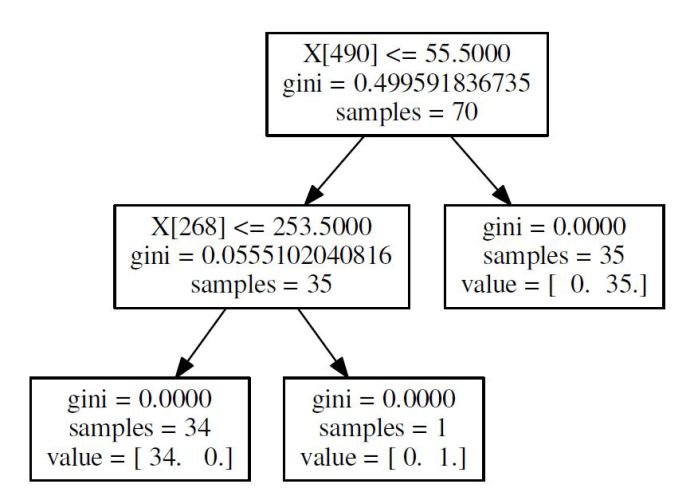
\includegraphics[scale=0.5,width=100mm]{./images/decision-tree-example.jpg}
  \caption{Example of a decision tree}
  \label{fig:abalone-decision-tree}
\end{figure}

Figure \ref{fig:abalone-decision-tree} \cite{decisionTreeExample} shows a decision tree classification.The top level node is called the root, The middle row shows internal nodes and the bottom row shows 2 leaf nodes. Decision trees are basically a series of if/else clauses. The edges (black lines in figure \ref{fig:abalone-decision-tree}) represent either true or false.

\subsection{Advantages of decision trees}

\begin{itemize}
  \item They are simple to use and visualize meaning they can easily be explained to other people.
  \item Not affected by non linear relationships. This is also a good advantage over linear regression.
  \item Makes minimal assumptions of the data.
  \item Not limited to numerical data like in linear regression
\end{itemize}

\subsection{Disadvantages of decision trees}

\begin{itemize}
  \item They can be very sensitive to changes in data. A slight change could result in an entirely different tree.
  \item There can be issues with out of sampling predictions because of their non-smooth nature.
  \item Execution speed is generally slower than linear regression.
\end{itemize}
